\documentclass[tikz,border=10pt]{standalone}
\usepackage{tikz}
\usetikzlibrary{arrows.meta,positioning}

\tikzset{
  rulebox/.style={draw=blue!70!black, line width=1.2pt, rounded corners=3pt, minimum width=7.8cm, minimum height=1.0cm, align=center, fill=none},
  note/.style={draw=orange!80!black, line width=1.2pt, rounded corners=3pt, minimum width=7.8cm, minimum height=1.0cm, align=center, fill=none}
}

\begin{document}
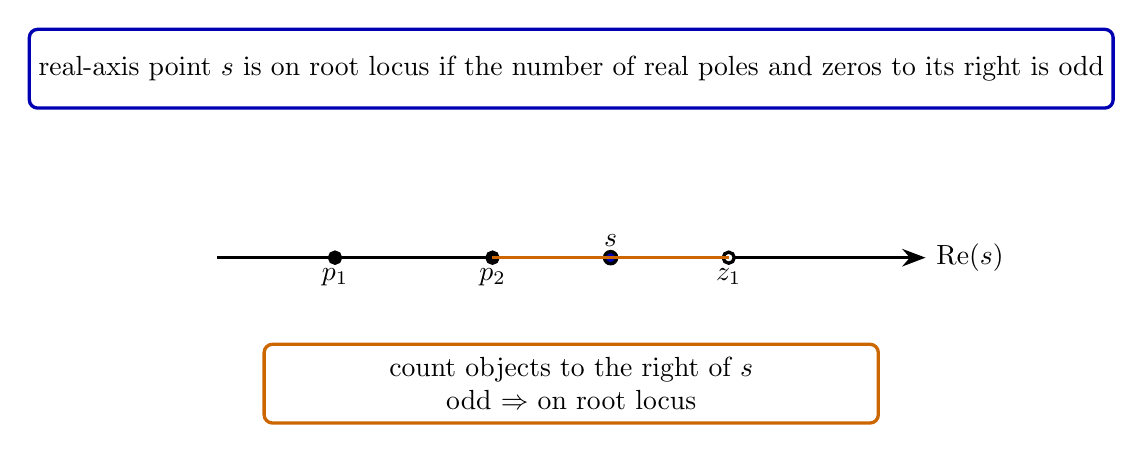
\begin{tikzpicture}[>=Stealth, line width=1.2pt]
  \node[rulebox] at (0,2.4) {real-axis point $s$ is on root locus if the number of real poles and zeros to its right is odd};
  \draw[->] (-4.5,0) -- (4.5,0) node[right] {$\mathrm{Re}(s)$};
  \draw[fill=black] (-3,0) circle (2pt) node[below] {$p_1$};
  \draw[fill=black] (-1,0) circle (2pt) node[below] {$p_2$};
  \draw[draw=black, fill=white, line width=1.2pt] (2,0) circle (2pt) node[below] {$z_1$};
  \draw[fill=blue!70!black] (0.5,0) circle (2.2pt) node[above] {$s$};
  \draw[very thick, orange!80!black] (-1,0) -- (2,0);
  \node[note] at (0,-1.6) {count objects to the right of $s$\\odd $\Rightarrow$ on root locus};
\end{tikzpicture}
\end{document}
